\documentclass[10pt]{extarticle}
\usepackage[a4paper]{geometry}
\usepackage[utf8]{inputenc}
\usepackage[french]{babel}
\usepackage{amssymb,amsthm,amsmath}
\usepackage{xltxtra}
\usepackage{stmaryrd}
\usepackage{graphicx}
\usepackage{listings}
\usepackage{color}
\lstset{
	extendedchars=true,
	showstringspaces=false,
	escapeinside=``,
	keywordstyle=\color{blue},
	commentstyle=\color[rgb]{0.133,0.545,0.133},
	columns=flexible,
	language=C++,
	tabsize=2,
	basicstyle=\normalsize\selectfont\ttfamily,
	numbers=left,
	frame=lines,
	breaklines=true
}
\geometry{
	left=15mm,
	right=7mm,
	top=7mm,
	bottom=15mm
}
\usepackage{multicol}
\setlength{\columnsep}{1cm}

\begin{document}

\tableofcontents


\section{Graphes}
\subsection{Dijkstra}
{\scriptsize\lstinputlisting{code/dijkstra.cpp}}

\subsection{Floyd-Warshall}
{\scriptsize\lstinputlisting{code/floydwarshall.cpp}}

\subsection{Bellman-Ford}
{\scriptsize\lstinputlisting{code/bellmanford.cpp}}

\subsection{Kruskal-Prim}
{\scriptsize\lstinputlisting{code/kruskalprim.cpp}}

\subsection{Parcours Eulerien}
{\scriptsize\lstinputlisting{code/eulertour.cpp}}

\subsection{SCC}
{\scriptsize\lstinputlisting{code/scc.cpp}}

\subsection{MCMF}
{\scriptsize\lstinputlisting{code/mcmf.cpp}}

\subsection{Min Cut}
{\scriptsize\lstinputlisting{code/mincut.cpp}}

\subsection{Couplage Maximal (biparti)}
{\scriptsize\lstinputlisting{code/bipartitematch.cpp}}

\subsection{Algorithme Hongrois}
{\scriptsize\lstinputlisting{code/hungarian.cpp}}

\subsection{BFS/DFS}
{\scriptsize\lstinputlisting{code/bfsdfs.cpp}}


\section{Strings}
\subsection{KMP}
{\scriptsize\lstinputlisting{code/kmp.cpp}}

\subsection{Boyer-Moore}
{\scriptsize\lstinputlisting{code/boyermoore.cpp}}

\subsection{Hashing}
{\scriptsize\lstinputlisting{code/hash.cpp}}

\subsection{Rabin-Karp}
{\scriptsize\lstinputlisting{code/rabinkarp.cpp}}

\subsection{Algorithme Z}
{\scriptsize\lstinputlisting{code/zalg.cpp}}

\subsection{Manacher (sous-palindrome le plus long)}
{\scriptsize\lstinputlisting{code/manacher.cpp}}


\section{Structures}
\subsection{Union Find}
{\scriptsize\lstinputlisting{code/unionfind.cpp}}

\subsection{Tableaux de Suffixes, LCP}
{\scriptsize\lstinputlisting{code/suffixarray.cpp}}

\subsection{Tries}
{\scriptsize\lstinputlisting{code/trie.cpp}}

\subsection{Arbres de segments}
\begin{figure}[h]
  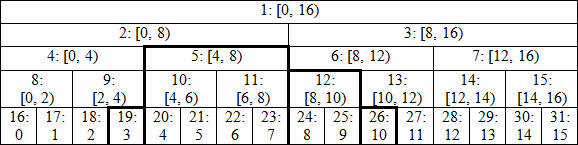
\includegraphics{code/segtree.png}
\end{figure}
{\scriptsize\lstinputlisting{code/segmenttree.cpp}}

\subsection{Treaps}
{\scriptsize\lstinputlisting{code/treap.cpp}}

\subsection{Arbres binaires indexés}
{\scriptsize\lstinputlisting{code/bit.cpp}}


\section{Géométrie}
\subsection{Enveloppe convexe}
{\scriptsize\lstinputlisting{code/convexhull.cpp}}

\subsection{Notes}
\begin{itemize}
  \item Sphere surface : $4\pi r^2$
  \item Cone surface : $\pi r^2 + \pi r h$
  \item Cone volume : $\frac{1}{3} \pi r^2 h$
  \item Cap surface : $2 \pi r h$
  \item Cap volume : $\frac{\pi h}{6}(3 a^2 + h^2)$
  \item Cap relation : $r = \frac{a^2 + h^2}{2h}$
\end{itemize}



\section{Arithmétique et Algèbre}
\subsection{Exponentation modulaire rapide}
{\scriptsize\lstinputlisting{code/fastexpmod.cpp}}

\subsection{DFT NTT, convolution}
{\scriptsize\lstinputlisting{code/dftntt.cpp}}

\subsection{Coefficients Binomiaux}
{\scriptsize\lstinputlisting{code/binomials.cpp}}

\subsection{Prochaine permutation (lexicographique)}
{\scriptsize\lstinputlisting{code/nextperm.cpp}}

\subsection{Enumeration de permutations}
{\scriptsize\lstinputlisting{code/enumperm.cpp}}

\subsection{Systèmes linéaires}
{\scriptsize\lstinputlisting{code/linear.cpp}}

\subsection{Décomposition LU}
{\scriptsize\lstinputlisting{code/determinant.cpp}}

\subsection{Inversion de matrice}
{\scriptsize\lstinputlisting{code/matinverse.cpp}}

\subsection{Multiplication chaînée}
{\scriptsize\lstinputlisting{code/matchain.cpp}}

\subsection{Simplexe}
{\scriptsize\lstinputlisting{code/simplex.cpp}}
 
\subsection{Algorithme d'Euclide Etendu}
{\scriptsize\lstinputlisting{code/exteuclid.cpp}}

\subsection{Kadane (sous tableau de somme max)}
{\scriptsize\lstinputlisting{code/kadane.cpp}}



\subsection{Notes}
 



\section{Bonus}
\subsection{Template}
{\scriptsize\lstinputlisting{code/template.cpp}}

\end{document}

